% Tipo de documento
\documentclass[16pt,spanish]{article}

% Ruta a la plantilla
\def \plpath{../plantilla}

% Paquetes
% Importaciones y paquetes %%%%%%%%%%%%%%%%%%%%%%%%%%%%%%%%%%%%%%

% Codificación
\usepackage[utf8]{inputenc}
\usepackage[spanish,activeacute]{babel}

% Paquetes extras
\usepackage{listings} % Trozos de código
\usepackage{graphicx} % Imágenes
\usepackage{fancyhdr} % Cabeceras
\usepackage{lscape}   % Apaisado
%\usepackage{hyperref} % Enlaces
\usepackage{float} % para que H funcione en figure
%\usepackage[left=2.5cm,top=2.5cm,right=2cm,bottom=2.5cm]{geometry}

% Configuración  %%%%%%%%%%%%%%%%%%%%%%%%%%%%%%%%%%%%%%%%%%%%%%%%%

\lstset{language=C++,
	showstringspaces=true}

% Figura centrada con \figura{proporcion}{ruta}{caption}{label}
% Ejemplo de uso: \figura{0.5}{img.png}{Boceto}{figura1}
% El argumento proporción es opcional y por defecto es el ancho del texto
%
%                 nargs   defaults
\newcommand{\figura}[4][1]{
\begin{figure}[H!] % Aparecerá justo donde está el código
	\centering
	     \includegraphics[width=#1\textwidth]{#2}
	\caption{#3}
	\label{#4}
\end{figure}
}

% Figura centrada y rotada 90º a la derecha
% con \figura{proporcion}{ruta}{caption}{label}
% Ejemplo de uso: \figura{0.5}{img.png}{Boceto}{figura1}
% El argumento proporción es opcional y por defecto es el ancho del texto
%
%                 nargs   defaults
\newcommand{\figuraApaisada}[4][1]{
\begin{figure}[H!] % Aparecerá justo donde está el código
	\centering
	     \includegraphics[width=#1\textwidth,angle=90]{#2}
	\caption{#3}
	\label{#4}
\end{figure}
}




%  Datos del documento a Editar %%%%%%%%%%%%%%%%%%%%%%%%%%%%%%%%%%%

% Título del documento
\def \titlename{Sion Tower}
\def \subtitlename{Documento de diseño}

% Autores separados por \and
\def \authorname{David Saltares Márquez}

% Versión de la revisión (En blanco para documentos nuevos)
\def \revname{1} % Ponemos un espacio para evitar errores en la cabecera.

% Fecha (En blanco para la fecha de hoy)
\def \datename{}

% Variables a usar para mantener un sistema consistente
\def \juego{\emph {Sion Tower} }
\def \jugador{\emph {Jugador} }
\def \wiki{\emph{IberOgre} }
\def \menu{\emph {Menú Principal} }
\def \selperfil{\emph {Selección de Perfil} }
\def \selhabilidad{\emph {Selección de Habilidades} }
\def \selnivel{\emph {Selección de Nivel} }
\def \nivel{\emph {Nivel} }
\def \finnivel{\emph {Fin de Nivel} }
\def \creditos{\emph {Créditos} }
\def \personaje{\emph {Personaje} }

% Configuración  %%%%%%%%%%%%%%%%%%%%%%%%%%%%%%%%%%%%%%%%%%%%%%%%%

\title{\titlename}
\author{\authorname}
%\date{\datename}

% Cabecera y pie del documento
\pagestyle{fancy}
%\renewcommand{\headrulewidth}{0.2pt}
%\fancyhead[HC]{ {\footnotesize \titlename} }
%\fancyhead[FR]{ {\footnotesize \thepage} }
%\fancyhead{}
%\fancyfoot{}


%%%%%%%%%%%%%%%%%%%%%%%%%%%%%%%%%%%%%%%%%%%%%%%%%%%%%%%%%%%%%%%%%

\begin{document}

% Portada %%%%%%%%%%%%%%%%%%%%%%%%%%%%%%%%%%%%%%%%%%%%%%%%%

% -*-portada.tex-*-
% Este fichero es parte de la plantilla LaTeX para
% la realización de Proyectos Final de Carrera, protejido
% bajo los términos de la licencia GFDL.
% Para más información, la licencia completa viene incluida en el
% fichero fdl-1.3.tex

% Fuente tomada del PFC 'libgann' de Javier Vázquez Púa

\begin{titlepage}

  \begin{center}

    
\includegraphics[scale=0.2]{logo_uca.png} \\
    
    \vspace{2.0cm}
    
    \LARGE{\textbf{ESCUELA SUPERIOR DE INGENIERÍA}} \\
    
    \vspace{1.0cm}
    
    \Large{\textbf{INGENIERÍA TÉCNICA EN INFORMÁTICA DE GESTIÓN}} \\
    
    \vspace{3.0cm}
    
    \Large{IBEROGRE, WIKI DE OGRE3D EN ESPAÑOL\\Y SION TOWER, VIDEOJUEGO DE ESTRATEGIA}\\
    
    \vspace{2.0cm}
    
    \Large{David Saltares Márquez} \\
  
    \vspace{0.5cm}

    \large{\today}
    
  \end{center}
\end{titlepage}


% Índice %%%%%%%%%%%%%%%%%%%%%%%%%%%%%%%%%%%%%%%%%%%%%%%%%%

\tableofcontents
\cleardoublepage

% Cambios en esta Revisión %%%%%%%%%%%%%%%%%%%%%%%%%%%%%%%%%%%%%%

%\section{Cambios}
%\label{sec:cambios} 


%\paragraph{}
%Cambios con respecto a versiones anteriores del documento.

%\begin{itemize}
%	\item {\bf Revision 1}
%		\begin{itemize}
%			\item Cambio1
%			\item Cambio2
%		\end{itemize}
%\end{itemize}

%%%%%%%%%%%%%%%%%%%%%%%%%%%%%%%%%%%%%%%%%%%%%%%%%%%%%%%%%%%%%%%%%

\section{Cambios}
\label{sec:cambios}
\paragraph{}
Cambios con respecto a versiones anteriores del documento.

\begin{itemize}
	\item {\bf Revision 1}
		\begin{itemize}
			\item Correcciones menores en todo el documento.
            \item Cambia el color de la bola de vida en la interfaz de verde
            a rojo para ganar contraste con respecto al azul de la magia.
		\end{itemize}
\end{itemize}

\clearpage

% Introducción %%%%%%%%%%%%%%%%%%%%%%%%%%%%%%%%%%%%%%

\section{Introducción}
\label{sec:introduccion}
\section{Proyecto propuesto}

\wiki\ es una documentación libre en formato wiki sobre desarrollo
de videojuegos en tres dimensiones utilizando el motor de renderizado
también libre \textsc{Ogre3D}. No sólo cubre el uso del conocido motor gráfico
sino que incluye documentación relacionada con otras bibliotecas y tecnologías
complementarias necesarias para el desarrollo de videojuegos. Además, tiene como objetivos
recordar y repasar los conceptos matemáticos fundamentales para continuar
estudiando esta disciplina como álgebra o geometría del espacio. Cada lección
intercalará conceptos teóricos y pequeños ejemplos prácticos para finalizar
con un paquete descargable completamente documentado que muestre una aplicación
práctica sobre dicha lección.\\

\juego\ es un videojuego de estrategia y acción en 3D de ambientación
fantástica cuyo objetivo es servir de ejemplo final a la wiki. Por supuesto,
hace uso de \textsc{Ogre3D} y otras tecnologías complementarias documentadas
en \wiki. En \juego\ controlamos a un joven hechicero iniciado que se ve obligado
a defender la Torre Sagrada de una invasión enemiga mientras sus compañeros
están celebrando un rito secreto en el exterior. Cada nivel es un piso
de la Torre y para poder avanzar tenemos que acabar con todos los enemigos
que atacan en oleadas la zona. Para hacerlo tendremos que emplear nuestra
energía mágica o maná en invocar proyectiles de diversa índole.
El videojuego debe estar completamente documentado para que los lectores
de \wiki\ tengan acceso directo a una aplicación práctica lo más realista posible
de la tecnología.\\


\section{Contexto}

En esta sección destacaremos la importancia de la industria del videojuego
empleando como escenario concreto España. Asimismo, haremos hincapié sobre
el éxito de los videojuegos 3D sobre los bidimensionales en términos de
mercado. Finalmente, realizaremos un pequeño repaso sobre qué es un motor
de videojuegos y adjuntaremos un breve comentario sobre algunos de ellos,
libres y privativos.\\

\subsection{Auge de los videojuegos 3D}

Es innegable que los videojuegos son un mercado en auge que está soportando
como pocos el efecto de la crisis económica mundial. En la sección
\ref{sec:videojuegos-industria} ofreceremos cifras que apoyan estas afirmaciones
dentro del contexto del mercado español.\\

Existe mucha discrepancia acerca de cuál es el primer videojuego de la
historia ya que la propia definición de videojuego resulta a la vez confusa.
Muchos consideran que Alenxander Douglas fue el padre del primer videojuego
moderno cuando en el año 1952 recreó en el computador EDSAC de la Universidad
de Cambridge una versión del popular tres en raya llamada OXO con gráficos
completamente primitivos (ver figura \ref{fig:oxo}) \cite{website:historia-videojuegos}.\\

\figura{oxo.jpg}{scale=0.9}{OXO, primer videojuego de la historia (1952)}{fig:oxo}{h}

Pasaron casi 30 años desde el primer videojuego moderno hasta que llegaron
los primeros videojuegos con sensación de profundidad en los años 80. Battlezone
(ver figura \ref{fig:battlezone}) era un videojuego de acción con tanques
y artillería para la consola Atari lanzado en 1980. Utilizaba vectores
verdes y rojos que delineaban el contorno de los objetos sobre el fondo
negro del escenario. Los videojuegos con gráficos vectoriales supusieron
un gran avance para la época ya que, con pocos recursos se podía conseguir
una aceptable sensación de profundidad \cite{website:historia-videojuegos}.\\

\figura{battlezone.jpg}{scale=0.6}{Battlezone, videojuego con gráficos vectoriales (1980)}{fig:battlezone}{h}

Los gráficos poligonales en tres dimensiones se popularizaron rápidamente
a finales de los años 80 y comienzos de los 90. No obstante, las técnicas
de programación no estaban lo suficientemente evolucionadas y, al aumentar
el detalle, aumentaba de manera exponencial la potencia de cálculo necesaria.
Alone in the Dark (ver figura \ref{fig:aloneinthedark}), publicado en 1992,
fue el primer videojuego completamente en 3D en cosechar un éxito importante,
además fue uno de los primeros en pertenecer al género de terror. Existen
otros muchos ejemplos de videojuegos que simulaban mundos 3D utilizando
un mundo 2D que se dibujaba en 3D (llamado a veces \emph{dos dimensiones y media}),
y que tuvieron éxito durante los 90 como Wolfenstein 3D (Id Software, 1992)
o Doom (Id Software, 1993) \cite{website:historia-videojuegos}.\\

\figura{aloneinthedark.jpg}{scale=0.5}{Alone in the Dark (PC - 1992)}{fig:aloneinthedark}{h}

A mediados de los 90 los gráficos 3D saltaron del PC a las consolas de
sobremesa. En 1994 Sega presentó Sega Saturn y Sony hizo lo propio con
PlayStation, en 1996 Nintendo lanzó al mercado Nintendo 64. La penetración
de estas consolas en el mercado fue tal que los gráficos en 3D llegaron a
millones de usuarios. PlayStation fue la consola más exitosa llegando a vender
100 millones de unidades. En esa época llegaron títulos revolucionarios
como el juego de infiltración y acción Metal Gear Solid (ver
figura \ref{fig:metalgearsolid}) o el plataformas Super Mario 64 (ver figura
\ref{fig:supermario64}). Los gráficos en 3D llegaron para quedarse \cite{website:historia-videojuegos}.\\

\figura{metalgearsolid.jpg}{scale=0.5}{Metal Gear Solid (PlayStation - 1998)}{fig:metalgearsolid}{h}

\figura{supermario64.jpg}{scale=0.35}{Super Mario 64 (Nintendo 64 - 1996)}{fig:supermario64}{h}

La siguiente generación de consolas llegó en el año 2000 con la PlayStation 2
de Sony. Un año más tarde Microsoft entró en el mercado con Xbox y Nintendo
lanzó Game Cube. PlayStation 2 se convirtió en la consola más vendida de 
la historia hasta el momento. Tanto en PC como en consolas de sobremesa, los gráficos
en 3D ya se habían consolidado. Llegaron títulos como God of War (ver figura
\ref{fig:godofwar}) y Half-Life 2 (ver figura \ref{fig:halflife2}) \cite{website:historia-videojuegos}.\\

\figura{godofwar.jpg}{scale=0.25}{God of War (PlayStation 2 - 2005)}{fig:godofwar}{h}

\figura{halflife2.jpg}{scale=0.25}{Half-Life 2 (PC - 2005)}{fig:halflife2}{h}

Otro hito en el mundo de los videojuegos tridimensionales fue su llegada
a las consolas portátiles, hasta entonces con insuficiente potencia. En 
2004 Nintendo lanzó su portátil Nintendo DS y poco después Sony respondió
con PlayStation Portable (PSP). La reducción de los procesadores permitió
que dispositivos de pequeño tamaño fueran capaces de mostrar en pantalla
un elevado número de polígonos y efectos. Actualmente este fenómeno está
tomando importancia en los dispositivos móviles iPhone y Android. Incluso
conocidos motores han llegado a iOS en demos técnicas como Epic Citadel
(ver figura \ref{fig:epiccitadel}) \cite{website:historia-videojuegos}.\\ 

\figura{epiccitadel.jpg}{scale=0.25}{Epic Citadel (iOS - 2009)}{fig:epiccitadel}{h}

El último paso han sido las consolas de la última generación Xbox 360 (2005),
Wii (2006) y PlayStation 3 (2006) y la llegada de la tecnología DirectX 11
al PC. Los entornos 3D se han hecho cada vez más grandes, los efectos
consiguen un mayor realismo y las físicas no difieren apenas de la realidad.
Las compañías luchan por estar a la vanguardia y los equipos más avanzados cuentan
con decenas de ingenieros especializados en campos muy concretos. Un ejemplo
de videojuego vanguardista podría ser Uncharted 2 (ver figura \ref{fig:uncharted2}) \cite{website:historia-videojuegos}.\\

\figura{uncharted2.jpg}{scale=0.8}{Uncharted 2 (PlayStation 3 - 2009)}{fig:uncharted2}{h}

Podemos concluir que los videojuegos tridimensionales han experimentado
una crecida exponencial a lo largo de los últimos años. Esto se debe a que
consiguen un mayor realismo e inmersión por parte del usuario dentro
del universo recreado.\\

% Videojuegos en auge
    % Dispositivos cada vez más capaces
    % Lucha tecnológica
    % LLegada de las 3D

\subsection{Los videojuegos como industria}
\label{sec:videojuegos-industria}

Si acudimos al último informe publicado por aDeSe \cite{pdf:adese2010}
(Asociación Española de Distribuidores y Editores de Software de
Entretenimiento), es decir, al correspondiente al pasado año 2010,
podemos percatarnos de la fuerza del sector en nuestro país. A pesar
del efecto provocado por la crisis económica que ha hecho disminuir el valor
de la industria un 5,2\% durante el último año, dicho valor llega a los 1.245
millones de euros. Además, la industria del videojuego copa el 50\% de todo el
mercado relacionado con el ocio visual e interactivo.\\

\figura{division-videojuegos.jpg}{scale=0.7}{División del sector de los videojuegos}{fig:division-videojuegos}{h}

Si prestamos atención a la figura~\ref{fig:division-videojuegos} podremos
observar que el sector del software sólo ha descendido un 0,38\% mientras
que el de los periféricos incluso ha crecido un 5,6\%. Por su parte, el sector de
las consolas ha disminuido un 13\%. Estas variaciones son comprensibles
ya que en 2010 las consolas actuales se aproximan poco a poco al final de
su ciclo de vida. Por ejemplo, la sucesora de la consola portátil Nintendo DS
\cite{website:nintendo-ds}, la recientemente lanzada Nintendo 3DS \cite{website:nintendo-3ds},
fue anunciada de forma oficial durante el año 2010. El aumento del segmento
de los periféricos ha podido crecer gracias al lanzamiento de Kinect \cite{website:kinect}
durante la campaña navideña del año 2010. Kinect es un sensor de movimiento
desarrollado por Microsoft compatible con la consola Xbox 360.\\

En definitiva, salvo pequeñas variaciones, la industria del videojuego
en España muestra salud y un gran potencial.\\

Para destacar la importancia de los videojuegos en 3D podemos recurrir
a la lista de los más vendidos en España durante el pasado año 2010 reflejada
en la tabla \ref{tab:ventas2010}.\\

\begin{table}[h]
  \begin{center}
  \begin{tabular}{| c |m{4cm}|m{2.5cm}|m{2cm}|m{3cm}|m{1cm}|}
    \hline
    \textbf{Puesto} & \textbf{Título} & \textbf{Plataforma} & \textbf{Género} & \textbf{Distribuidor} & \textbf{¿3D?} \\
    \hline
    1 & Call of Duty: Black Ops & PlayStation 3 & Acción & Activision Blizzard & Sí \\
    \hline
    2 & New Super Mario Bros. & Wii & Plataformas & Nintendo & Sí \\
    \hline
    3 & Wii Fit Plus & Wii & Fitness & Nintendo & Sí \\
    \hline
    4 & Gran Turismo 5 & PlayStation 3 & Conducción & Sony & Sí \\
    \hline
    5 & Wii Party & Wii & Party Game & Nintendo & Sí \\
    \hline
    6 & FIFA 11 & PlayStation 3 & Deportivo & Electronic Arts & Sí \\
    \hline
    7 & Pro Evolution Soccer 2011 & PlayStation 3 & Deportivo & Konami & Sí \\
    \hline
    8 & Super Mario Galaxy 2 & Wii & Plataformas & Nintendo & Sí \\
    \hline
    9 & God of War III & PlayStation 3 & Acción & Sony & Sí \\
    \hline
    10 & Art Academy & Nintendo DS & Habilidad & Nintendo & No \\
    \hline
    11 & Mario Kart & Wii & Conducción & Nintendo & Sí \\
    \hline
    12 & Formula 1 2010 & PlayStation 3 & Conducción & Warner Interactive & Sí \\
    \hline
    13 & Call of Duty: Modern Warfare 2 & PlayStation 3 & Acción & Activision Blizzard & Sí \\
    \hline
    14 & Wii Sports Resort & Wii & Deportes & Nintendo & Sí \\
    \hline
    15 & Red Dead Redemption & PlayStation 3 & Acción & Take 2 & Sí \\
    \hline
    16 & Pokémon Soulsilver & Nintendo DS & RPG & Nintendo & No \\
    \hline
    17 & Assassin's Creed: La Hermandad & PlayStaton 3 & Acción & Ubisoft & Sí \\
    \hline
    18 & Wii Play & Wii & Party Game & Nintendo & Sí \\
    \hline
    19 & Pokémon Heartgold & Nintendo DS & RPG & Nintendo & No \\
    \hline
    20 & Starter Pack & PlayStation 3 & Party Game & Sony & Sí \\
    \hline
  \end{tabular}
\end{center}
\caption{Tabla de los 20 videojuegos más vendidos en España durante el año 2010}
\label{tab:ventas2010}
\end{table}

Como puede observarse, un 85\% de los juegos más vendidos en España durante
el año 2010 en cualquier plataforma son en tres dimensiones. Dicha cifra ya
resulta un claro indicador del atractivo que suponen las 3D para la comunidad
de usuarios. No obstante, si tenemos únicamente en cuenta los títulos para
consolas de sobremesa (17 entre los 20 más vendidos), vemos que el 100\%
de ellos utilizan gráficos tridimensionales.\\

% Economía (informe español aDeSe)

\subsection{Motores de videojuegos}

Como indica la publicación Game Engine Architecture de Jason Gregory
\cite{greg09} el término \emph{motor de videojuegos} apareció a mediados
de los años 90 con el videojuego de acción en primera persona Doom
\cite{website:doom} de Id Software (ver figura \ref{fig:doom}). Fue el
primer videojuego cuya arquitectura estaba bien definida y separaba
componentes como el motor de renderizado, el sistema de audio, la detección
de colisiones y los recursos artísticos. Esto permitió que los desarrolladores
pudiesen reutilizar estos elementos para lanzar nuevos productos distintos
al original. Podían cambiar armas, niveles y vehículos con ninguno o
pocos cambios al motor.\\

\figura{doom.jpg}{scale=0.3}{Doom (PC - 1993)}{fig:doom}{h}

Fue entonces cuando nació lo que se conoce como la comunidad del \emph{modding}.
Usuarios y profesionales que se dedican a modificar juegos aprovechando
la independencia del motor de los recursos. Estos arreglos pueden ir desde
modificar reglas de juego, añadir elementos hasta incluso crear un juego
radicalmente diferente al original. A finales de la década de los 90
ya se desarrollaban motores con estas modificaciones en mente. Un ejemplo
es Quake III Arena \cite{website:quakeIII} de Id Software (ver figura
\ref{fig:quakeIII}) y su lenguaje de scripting Quake C.\\

\figura{quakeIII.jpg}{scale=0.3}{Quake III Arena (PC - 1999)}{fig:quakeIII}{h}

Hoy en día es muy común que muchas compañías pequeñas no puedan permitirse
económicamente el desarrollo de su propio motor. Por ello, adquieren licencias
de motores de compañías externas para comenzar sus proyectos. A pesar de que
dichas licencias conllevan un desembolso importante, suele ser más asequible
que el desarrollo completo del motor.\\

La línea que separa lo que es un motor de videojuegos de lo que no lo es
es muy difusa. Un motor podría saber cómo dibujar un personaje específico
mientras que otro simplemente recibiría una colección de vértices y triángulos
de un fichero en memoria secundaria. Por tanto, el segundo motor sería
más generalista que el segundo y más reutilizable. Cuando un motor incluye
lógica de juego y elementos muy concretos dentro de su código fuente, es 
prácticamente imposible reutilizarlo para otro propósito. La situación opuesta
tampoco se da, no existe un motor capaz de ser óptimo en cualquier situación.
Hay algunos que están preparados para mostrar escenarios gigantescos con bajo
nivel de detalle y miles de personajes en pantalla mientras que otros
se centran en entornos limitados con un nivel de detalle y efectos impresionante.\\

\figura{abaddon.jpg}{scale=0.17}{Videojuego libre Abaddon}{fig:abaddon}{H}

Afortunadamente, existen motores libres como \textsc{Ogre3D} (\textit{Object
Oriented Graphics Rendering Engine} o motor gráfico de renderizado orientado
a objetos). Básicamente es una biblioteca compatible con el lenguaje de
programación C++ que abstrae las funcionalidades de bajo nivel de DirectX \cite{website:directx}
y OpenGL \cite{website:opengl} para comunicarse con el hardware. Su versión
1.0 de nombre en clave Azathoth fue lanzada en 2005 y desde entonces ha cosechado
grandes éxitos como el premio al proyecto del mes en SourceForge. Únicamente
proporciona el sistema de renderizado (dibujado de una escena 3D en patalla)
por lo que es necesario implementar otros subsistemas o recurrir a otras bibliotecas
(colisiones, audio, entrada del usuario, red, etc) \cite{junk06}.\\

\figura{stuntrally.jpg}{scale=0.25}{Videojuego libre Stunt Rally}{fig:stuntrally}{H}

Su licencia permisiva (MIT) ha permitido la creación tanto de juegos libres
como comerciales y cerrados. Abaddon (figura \ref{fig:abaddon}) y Stunt Rally (figura
\ref{fig:stuntrally}) son videojuegos libres de géneros muy distintos (rol y conducción
respectivamente) que han sido desarrollados utilizando \textsc{Ogre3D}, lo que
demuestra su enorme versatilidad. Asimismo, como títulos cerrados
podemos mencionar a Torchlight (figura \ref{fig:torchlight}) y a Victory The Age of Racing
(figura \ref{fig:victory}) \cite{junk06}. \\

\figura{torchlight.jpg}{scale=0.25}{Torchlight (Windows, Mac - 2009)}{fig:torchlight}{H}

\textsc{Ogre3D} cuenta con una arquitectura (figura \ref{fig:aquitectura-ogre})
modular extensible a través de plugins. Si una característica necesaria para
nuestro proyecto no viene incluida en el motor es posible implementarla
e integrarla sin demasiados problemas. Por supuesto, también es recomendable
acudir a su excelente comunidad ya que es probable que lo que busquemos esté
hecho y pueda ser reutilizado. Queda patente por las capturas de pantalla
que \textsc{Ogre3D} es un motor gráfico moderno con grandes capacidades
\cite{junk06}.\\

\figura{victory.jpg}{scale=0.3}{Victory (Windows - 2011)}{fig:victory}{H}

Actualmente, \textsc{Ogre3D} es uno de los mejores motores gráficos libres
que existen. Si bien es cierto que su potencia y extensibilidad hacen que
la curva de aprendizaje sea elevada, el hecho de tomar elementos similares
al de otros motores ampliamente utilizados en la industria lo hace ideal
para el aprendizaje a aquellos interesados en la materia de forma profesional.\\

\figura{arquitectura-ogre.jpg}{scale=0.9}{Arquitectura de \textsc{Ogre3D}}{fig:aquitectura-ogre}{H}


\section{Motivaciones}
\label{sec:motivaciones}

Comenzar a utilizar una tecnología desconocida como \textsc{Ogre3D} o cualquier
otra siempre entraña cierta dificultad y, si le añadimos la barrera del 
idioma, aún más. La principal motivación para embarcarme en la confección
de una documentación sobre desarrollo de videojuegos en 3D como es \wiki\
ha sido la ausencia de información al respecto en castellano. Hasta
ahora sólo se habían publicado pequeños tutoriales en blogs personales
pero no existía una plataforma de aprendizaje y documentación
equivalente a la wiki oficial de \textsc{Ogre3D} \cite{website:ogre3d-wiki}
en español.\\

\textbf{Diseño de Videojuegos} es una asignatura optativa de tercer curso
de la titulación Ingeniería Técnica en Informática de Sistemas dentro
de la Universidad de Cádiz. En dicha asignatura los alumnos se organizan
en grupos de tres con el objetivo de desarrollar un juego sencillo en dos
dimensiones durante el cuatrimestre. Las únicas restricciones son que
el videojuego resultante debe ser completamente libre y que han de utilizar
la forja de código de RedIRIS \cite{website:rediris} junto a \textit{Subversion} 
\cite{website:svn} como sistema de control de versiones. Los alumnos de la
asignatura suelen utilizar bibliotecas libres para desarrollar aplicaciones
multimedia en dos dimensiones como \textsc{libSDL} \cite{website:sdl} o
\textsc{Gosu} \cite{website:gosu}. Toda la documentación estaba en inglés, pero
para la primera de ambas bibliotecas ya se publicó una excelente documentación
en castellano en formato wiki llamada \textbf{Wikijuegos} \cite{website:wikijuegos}.\\

De esta manera, los alumnos podían seguir la extensa documentación sin
muchos problemas a la vez que trabajaban sobre los múltiples ejemplos
aprendiendo conceptos que, más tarde, incorporarían en sus proyectos. No 
obstante, cuando terminasen la asignatura no disponían de una bibliografía
en español para continuar ampliando sus conocimientos en el terreno de las
tres dimensiones.\\

Cualquiera que desee iniciarse en el mundo del desarrollo de aplicaciones
en tiempo real en tres dimensiones (ya sean videojuegos o no) debe adquirir
o recordar una fuerte base de matemáticas. Principalmente, son necesarios
conocimientos relativos a álgebra lineal, trigonometría y geometría del espacio.
En numerosas ocasiones también nos vemos obligados a utilizar
conceptos de física como óptica, cinemática, dinámica, etc. Lo usual es que
el aprendiz se va obligado a recurrir a varias fuentes de información
no conexas entre sí. Una motivación importante era proporcionar en un sólo
lugar, el uso de una tecnología y los conocimientos matemáticos necesarios
para trabajar con ella.\\

La wiki oficial de \textsc{Ogre3D} \cite{website:ogre3d-wiki} y el resto
de documentación tanto accesible en la red como impresa se centran principalmente
en el desarrollo para plataformas cerradas como es Windows con herramientas
privativas tales como Microsoft Visual Studio. Lo natural en una documentación
libre es tratar de ofrecer un soporte multiplataforma utilizando herramientas
libres como, por ejemplo, el compilador GNU GCC \cite{website:gnu-gcc}.\\

Mi interés en aprender a desarrollar videojuegos en tres dimensiones fue el
motor principal que me llevó a desarrollar \juego. Son tantos los conceptos
nuevos, las tecnologías desconocidas y las aproximaciones diametralmente
opuestas que las posibilidades de adquirir conocimiento son enormes. En cualquier
caso, \wiki\ necesitaba un gran ejemplo final que pusiera en práctica todo
lo visto a lo largo de las lecciones. Una puesta en práctica lo más cercana
a la realidad completamente documentada para que cualquier lector pudiera
comprender de primera mano cómo se desarrolla un videojuego en 3D (aunque
sea de pequeñas dimensiones).\\

La idea de que \juego\ tuviera componentes fácilmente reutilizables por
los lectores interesados también resultaba muy atractiva. La posible
distribución por separado de subsistemas libres documentados en detalle
como el motor de colisiones quizás fuera útil a otros usuarios que
estuviesen comenzando.\\

Es posible resumir las motivaciones que me han llevado a desarrollar este
proyecto en cubrir el vacío de documentación en castellano, el hecho de que
pocas fuentes hagan hincapié en herramientas libres y el deseo personal
de aprender a crear videojuegos en tres dimensiones.\\


\section{Objetivos}
\label{sec:objetivos}

El objetivo principal del proyecto viene extraído de forma lógica de las
motivaciones (sección \ref{sec:motivaciones}). Con \wiki\ se pretende
crear una documentación libre que facilite el aprendizaje del desarrollo
de videojuegos en 3D. Por su parte, con \juego\ se desea proporcionar una 
aplicación práctica ampliamente documentada y accesible de todo el contenido
tratado en la wiki.\\

\wiki\ debe cumplir con los siguientes requisitos básicos:

\begin{itemize}
    \item El contenido debe abarcar los principales subsistemas de
    \textsc{Ogre3D} de forma que el lector sea capaz de desarrollar aplicaciones
    en tres dimensiones y pueda ampliar sus conocimientos de forma autónoma.
    Para ello deben darse pocos conceptos por supuestos y explicar los temas
    más básicos en primer lugar para ir ascendiendo en complejidad de forma
    progresiva. A pesar de ello, para continuar las lecciones será imprescindible
    tener una mínima experiencia con videojuegos en dos dimensiones.
    \item Debe proporcionarse una sección con los contenidos matemáticos
    mínimos sobre geometría del espacio para comprender el resto de material
    de la wiki. No se pretende publicar material educativo sobre matemáticas
    en el sentido más estricto sino ofrecer los conceptos con un enfoque
    eminentemente práctico. El nivel ofrecido será similar al impartido
    en segundo de bachillerato.
    \item \textsc{Ogre3D} es simplemente un motor de renderizado y no
    proporciona subsistemas imprescindibles para la creación de un videojuego
    como entrada de usuario o sonido. En la documentación debe existir una
    sección para otras tecnologías que cubran bibliotecas complementarias
    a \textsc{Ogre3D}.
    \item Emplear una aproximación lo más práctica posible. Deben intercalarse
    los contenidos teóricos del desarrollo de cada lección con pequeños
    ejemplos. Para finalizar cada artículo debe adjuntarse un ejemplo de mayores
    dimensiones que evidencie las técnicas comentadas en el texto.
    \item Prestar especial atención y soporte a herramientas de desarrollo
    libre y multiplataforma.
    \item Ofrecer técnicas y buenas prácticas para el desarrollo de software
    multiplataforma. Todas las herramientas y bibliotecas empleadas lo son
    y carecería de sentido que el código escrito por los lectores fuera
    dependiente de una arquitectura o plataforma sin necesidad de ello.
    \item Construir una comunidad que colabore de forma activa con la
    documentación probado ejemplos, informando de errores encontrados y
    creando nuevo contenido de interés para el resto de usuarios.
\end{itemize}

\juego\ debe cumplir con los siguientes requisitos:

\begin{itemize}
    \item Servir de ejemplo lo más cercano a la realidad posible de un
    desarrollo de videojuego 3D. Es muy habitual terminar de leer documentación,
    hacer pequeñas prácticas pero no sentirse capaz de embarcarse en un
    proyecto de mayores dimensiones utilizando la misma tecnología. Para ello
    es imprescindible que se documente cada fase del desarrollo.
    \item Crear un pequeño motor orientado a la producción de contenido, una
    de las prácticas mejor valoradas. Cualquier diseñador podría añadir
    niveles al juego sin necesidad de tocar el código fuente ni recompilarlo.
    \item Convertirse en un ejemplo de trabajo con un equipo multidisciplinar.
    En un videojuego profesional deben trabajar juntos desde unas pocas personas
    hasta varios centenares por lo que la coordinación entre profesionales
    de distintas áreas es muy importante. Será necesario encontrar artistas
    relacionados con el modelado 3D, música y efectos de sonido.
    \item No sólo debe ser útil a los interesados en el desarrollo sino también
    de cara al usuario final. \juego\ debe ser cómodo de utilizar, intuitivo
    y divertido.
    \item Crear subsistemas independientes del videojuego reutilizables
    por la comunidad de usuarios. Por supuesto, deben venir acompañados
    de la documentación pertinente: dependencias, instalación, uso y licencia.
\end{itemize}

\section{Sobre este documento}

La presente memoria de \textbf{Proyecto Fin de Carrera} posee la siguiente
estructura en capítulos y apéndices:

\begin{itemize}
    \item En el capítulo \ref{chap:introduccion} que actualmente nos ocupa,
    se hace una breve introducción sobre el contexto en el que nos situamos.
    Se ofrece una visión del mundo de los videojuegos como industria y se
    habla sobre el actual mercado de los motores para videojuegos.
    Finalmente se evidencia la necesidad de documentación en castellano
    sobre uno de estos motores libres (\textsc{Ogre3D}) y se adjuntan el
    resto de motivaciones y objetivos relacionados con el proyecto.
    \item En el capítulo \ref{chap:calendario} se expone la organización
    temporal de todo el desarrollo a través de un diagrama de Gantt. Más 
    adelante se comenta brevemente cada una de las tareas que conforman
    la planificación.
    \item En el capítulo \ref{chap:desarrollo-iberogre} se documenta
    en profundidad el desarrollo de la wiki \wiki. Se incluye la metodología
    utilizada, el análisis de requisitos, el diseño de la plataforma, los
    detalles de la redacción de los artículos, la implementación de los
    ejemplos y las pruebas realizadas.
    \item En el capítulo \ref{chap:desarrollo-siontower} se refleja el proceso
    de desarrollo para el videojuego \juego. Comenzando con el documento
    de diseño, se sigue con la fase de análisis, diseño e implementación.
    Se hace especial hincapié en los subsistemas que entrañan mayor complejidad
    como el sistema de detección de colisiones. Se finaliza con las pruebas
    realizadas.
    \item En el capítulo \ref{chap:conclusiones} se hace una breve reflexión
    personal seguida de otra técnica tratando de aglutinar los conceptos
    aprendidos, la riqueza que ha proporcionado la experiencia y lo que
    podrá aportar a la comunidad. Finalmente se termina con un pequeño
    listado sobre las posibilidades de ampliación del proyecto.
    \item En el apéndice \nameref{chap:software} se hace un repaso por todas
    las herramientas empleadas a lo largo del desarrollo
    del proyecto. Asimismo, se adjuntan comentarios y las razones de su uso.
    \item En el apéndice \nameref{chap:manual} se incluye un completo manual
    de usuario para \juego. El documento contiene la introducción a la historia,
    personajes y hechizos del juego así como una completa guía de instalación
    en sistemas GNU/Linux y Windows. Posteriormente se detallan las mecánicas
    de juego y los controles en detalle. Finalmente se añade una completa guía
    para añadir niveles adicionales a \juego\ creados con la herramienta
    \textit{Blender}.
    \item En el apéndice \nameref{chap:comunidad} se realiza un recorrido
    por las actividades relacionadas con el presente proyecto y la
    comunidad del Software Libre. Se mencionan actividades como el
    \textbf{V Concurso Universitario de Software Libre} y los medios de difusión
    utilizados.
\end{itemize}

\clearpage

\section{Mecánicas de juego}
\label{sec:mecanicas}
\paragraph{}
En esta sección entraremos más en detalle en lo que a las mecánicas de
\juego se refiere. Se comentarán todos los pilares que fundamentan su
jugabilidad y se detallarán las acciones que podrá llevar a cabo el jugador
dentro de una partida típica. Además, se ofrecerá una lista con los personajes
del juego (tanto protagonista como enemigos), habilidades, objetos etc.
Por último, se modelará el mundo en el plano de movimiento, físicas y
detección de colisiones.


\subsection{Jugabilidad}
\label{sec:mec-jugabilidad}

\paragraph{Niveles}
Cada nivel de \juego es un piso de la torre sagrada (en orden ascendente)
que nuestro joven mago debe defender. Escenarios interiores
reducidos con varias entradas y un objeto valioso (reliquia) en el centro.
Los invasores acceden al nivel por las puertas y debemos impedir que alcancen
el objeto. Los niveles tendrán obstáculos, sobre todo mobiliario,
que dificultará o el tránsito por algunas zonas. Habremos vencido cuando
las oleadas de enemigos (previamente establecidas) hayan cesado.

\paragraph{Varios focos}
Nuestro personaje se verá sobrepasado por la entrada simultánea de enemigos
en el nivel. La posibilidad de moverse con libertad por las zonas libres
del escenario le permitirá atender los puntos de entrada según el criterio
del \jugador. El movimiento de los personajes será sobre un plano (el suelo)
aunque más adelante se darán más detalles sobre el movimiento.

\paragraph{Intensidad}
La dificultad de \juego viene dada por la cantidad de enemigos asaltando
el nivel, su fortaleza y la distancia entre los distintos puntos de acceso.
Entre niveles la intensidad y dificultad de las partidas irá aumentando en
consonancia al gráfico que se muestra a continuación.

\begin{figure}[H]
    \centering
        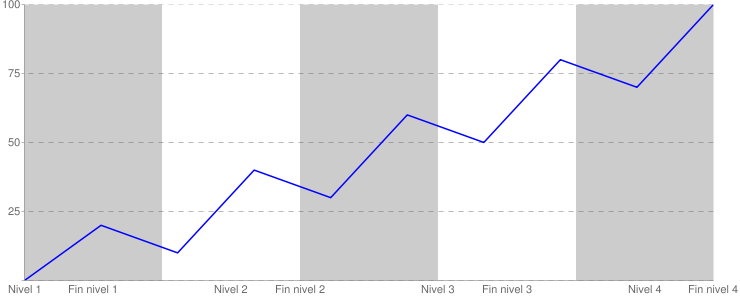
\includegraphics[width=12cm]{img/intensidad.png} 
    \caption{Intensidad de juego a lo largo de los niveles}
    \label{img:intensidad}
\end{figure}

\paragraph{Trampas}
Las trampas conforman una de las herramientas del \jugador para hacer frente
a la invasión. Consumen parte de los recursos del protagonista y pueden
ser útiles para impedir el avance del enemigo o para infligirle daño
si se éste se topa con una. Son elementos estáticos que coloca manualmente
el \jugador.

\paragraph{Habilidades}
Las habilidades inciden en el componente de acción de \juego de forma que
se aleja del clásico Tower Defense. El protagonista debe acudir al foco de
acción que considere oportuno para utilizar hechizos directos que dañarán
a sus enemigos. Existirán varios tipos de habilidades y hechizos cuya efectividad
dependerá de las características del enemigo.

\paragraph{Recursos limitados}
El \jugador no podrá dedicarse a lanzar hechizos y colocar trampas sin
llevar una táctica concreta. El protagonista cuenta con un potencial limitado
(no olvidemos que es un simple iniciado) y debe administrarlo racionalmente.
El protagonista sólo podrá utilizar una habilidad concreta si sus puntos de
\emph{Energía mágica} superan al coste de dicha habilidad. Como veremos en secciones
posteriores, ciertas trampas y habilidades funcionan mejor que otras según
el enemigo y el escenario. Por ejemplo: un hechizo de hielo será mucho más
efectivo contra una criatura débil ante ese elemento que contra otra que lo resista.
Además, un obstáculo de reducido tamaño sólo funcionará si se coloca en un
pasillo de tamaño reducido. El componente táctico es primordial y cobrará mucha
importancia en el desarrollo de una partida.

\paragraph{Progresión del jugador}
El \jugador progresará a medida que avanza por los niveles consiguiendo
nuevas habilidades. De esta forma el \jugador no sólo se verá recompensado
por completar niveles sino por el hecho de que su personaje sea más poderoso.

\paragraph{Planificación de la batalla}
El \jugador tendrá a su disposición un conjunto más o menos amplio de habilidades,
según estas se hayan desbloqueado o no. No obstante, las pobres habilidades
del protagonista le impiden utilizarlas todas al mismo tiempo. Antes de cada
nivel, el \jugador deberá elegir únicamente 5. Con esta decisión se pretende
aumentar el componente táctico de \juego. Por supuesto, de cara al siguiente
nivel, el \jugador podrá volver a elegir el subconjunto de habilidades
que considere oportuno.

\subsection{Flujo de juego}
\label{sec:mec-flujo}

\paragraph{}
A lo largo de esta sección se detallará el transcurso de una partida típica
a \juego. Se comentarán los pasos que ha de seguir el \jugador desde el arranque
del juego hasta completar un nivel completo. Poco a poco vamos desgranando
el funcionamiento exacto del juego, en esta sección describimos las mecánicas.
Más adelante se definirá el contenido de cada pantalla.

\paragraph{}
El \jugador inicia \juego y se le presenta el \menu. Si desea iniciar una
partida el \jugador seleccionará la opción \emph{Jugar}. \juego soporta
varias partidas guardadas en forma de perfiles. En la
siguiente pantalla el \jugador seleccionará el perfil que desee. Si no
cuenta con un perfil creado podrá crear uno nuevo. Entonces,
el \jugador podrá elegir cualquiera de los niveles que haya desbloqueado
en la pantalla de \selnivel.

\paragraph{}
Los niveles se organizan de forma secuencial y cada vez que se completa
uno, se desbloquea el siguiente. Luego, hay que seleccionar el conjunto
de habilidades y trampas de las que dispondrá el protagonista en el transcurso
del nivel (\selhabilidad). El \jugador podrá seleccionar 5 de ellas llenando los slots
(casillas) disponibles

% Desarrollo de una partida
\paragraph{}
El personaje comienza el nivel en el centro del piso y se le advertirá al
\jugador que las oleadas están próximas. Deberá proteger una zona que albergará
alguna reliquia mágica. El \jugador será derrotado si las bestias la alcanzan
o si acaban con la vida del protagonista. Poco a poco aparecerán enemigos
por las entradas del nivel. El \jugador podrá seleccionar en cualquier
momento una de las habilidades o trampas disponibles. Sólo
podrá utilizarlas si su nivel de energía se lo permite. La energía mágica
se irá recargando con el paso del tiempo. Si hemos seleccionado una habilidad,
al pulsar el botón de ataque, ésta será proyectada en la dirección actual.
En cambio, si tenemos una trampa seleccionada, la colocaremos en la posición
deseada. Cuando abatimos a un enemigo recibiremos puntos que nos ayudarán
a desbloquear más habilidades.

\paragraph{}
Si el personaje muere o los enemigos alcanzan la zona que debemos proteger
se mostrará un mensaje de \emph{`Game Over'} y el nivel se reiniciará. No
hay un número determinado de vidas, el \jugador puede repetir un escenario
cuantas veces necesite.

% Fin del nivel
\paragraph{}
Cuando hemos acabado con las oleadas de enemigos del nivel actual
aparece un cartel de \emph{`Victoria'} indicándole al \jugador
que ha completado el piso. Tras la pantalla de \nivel vamos a la de \finnivel.
En ella se nos comunica el progreso que hemos realizado y si hemos
conseguido desbloquear una nueva habilidad. En tal caso, dicha habilidad
aparecerá disponible la próxima vez que acudamos a la pantalla de \selhabilidad.
En el momento en el que el \jugador acepte volveremos a la pantalla de \selnivel con un nuevo
nivel disponible.

\paragraph{}
Cuando lo desee, el \jugador podrá regresar a pantallas anteriores o al
\menu. Más adelante se mostrarán todas la posibilidades de flujo
entre pantallas.

\subsection{Personajes}
\label{sec:mec-personajes}

\paragraph{}
En esta sección procederemos a enumerar y describir todos los personajes
de \juego así como sus habilidades y comportamiento. 

\paragraph{}
Existen habilidades y enemigos afines a algún elemento. Tenemos tres elementos
que se sitúan en forma de triángulo. De esta forma uno es efectivo contra
un segundo pero débil ante un tercero. Dicho triángulo se expone en el siguiente
gráfico:

\begin{figure}[H]
    \centering
        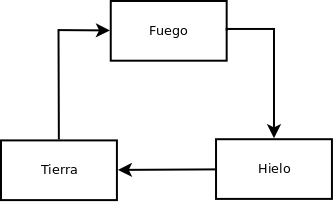
\includegraphics[width=5cm]{img/elementos.png} 
    \caption{Elementos del juego y su relación}
    \label{img:elementos}
\end{figure}

\subsubsection{Protagonista}

% Descripción
\paragraph{Descripción}
\personaje es el protagonista de \juego. Es un iniciado en la torre de los
magos y su misión es protegerla mientras sus compañeros acuden a un rito sagrado.
\personaje es joven, simpático y tiene un carácter apasionado, propio de un
iniciado. Su apariencia es muy sencilla, no lleva ropas de lujo ni adornos dado
su status en la jerarquía de la comunidad mágica. Va armado con un báculo
de iniciado.

% Concept art

\begin{itemize}
    \item \textbf{Vida inicial}: 100 (se restaura en cada nivel)
    \item \textbf{Magia inicial}: 100 (se restaura en cada nivel)
    \item \textbf{Experiencia inicial}: 0
    \item \textbf{Velocidad}: 20
\end{itemize}

% Habilidades
\paragraph{Habilidades}
La siguiente tabla muestra la lista de habilidades de \personaje junto
con una descripción, su coste en energía mágica y la experiencia necesaria
para desbloquearlas.

\begin{table}[H]
    \centering
        \begin{tabular}{| p{2.6cm} | p{7cm} | p{2cm} | p{2cm} | p{2cm} |}
            \hline
            \textbf{Habilidad} & \textbf{Descripción} & \textbf{Daño} & \textbf{Magia} & \textbf{Experiencia}\\
            \hline
            Bola de fuego & Hechizo a distancia del elemento \emph{fuego} & 30 & 20 & 0  \\
			\hline
            Furia de Gea & Ataque a distancia del elemento \emph{tierra} & 30 & 20 & 0  \\
			\hline
            Ventisca & Hechizo a distancia del elemento \emph{hielo} & 30 & 20 & 500  \\
			\hline
        \end{tabular}
    \caption{Hechizos del protagonista}
    \label{tab:hechizos}
\end{table}

% Trampas
\paragraph{Trampas}
La siguiente tabla muestra la lista de trampas de \personaje junto
con una descripción, su coste en energía mágica y la experiencia necesaria
para desbloquearlas.

\begin{table}[H]
    \centering
        \begin{tabular}{| p{2.7cm} | p{7cm} | p{2cm} | p{2cm} | p{2cm} |}
            \hline
            \textbf{Trampa} & \textbf{Descripción} & \textbf{Daño} & \textbf{Magia} & \textbf{Experiencia}\\
            \hline
            Panel de pinchos & Crea un panel en el suelo por tiempo limitado con peligrosos pinchos & 10 & 40 & 0  \\
			\hline
            Muro mágico & Crea un muro semitransparente que impide temporalmente el paso de enemigos & - & 40 & 800  \\
			\hline
            Señuelo & Crea un espejismo de la reliquia del nivel lo que provoca que los enemigos se despisten temporalmente & - & 70 & 1000  \\
			\hline
        \end{tabular}
    \caption{Trampas del protagonista}
    \label{tab:trampas}
\end{table}

\subsubsection{Goblin}

% Descripción
\paragraph{Descripción}
Enemigo básico sin ninguna afinidad elemental. Clásica criatura verde, desagradable
y de baja estatura. Va armado con una tosca espada corta y un burdo taparrabos.
Acuden en gran número (su gran ventaja), son ágiles pero no tienen grandes
habilidades en combate.

\begin{itemize}
    \item \textbf{Vida}: 60
    \item \textbf{Ataque}: 15
    \item \textbf{Velocidad}: 20
    \item \textbf{Afinidad elemental}: ninguna
\end{itemize}

\subsubsection{Diablillo}

% Descripción
\paragraph{Descripción}
Criatura del averno de estatura ligeramente superior al Goblin. Cuenta con
la cola y los cuernos clásicos de los demonios. No lleva ropa y su rojo
oscuro de piel le confiere un aspecto más despiadado. Ataca con sus afiladas
garras y no necesita ningún tipo de arma adicional.

\begin{itemize}
    \item \textbf{Vida}: 70
    \item \textbf{Ataque}: 25
    \item \textbf{Velocidad}: 20
    \item \textbf{Afinidad elemental}: fuego
\end{itemize}

\subsubsection{Gólem de hielo}

% Descripción
\paragraph{Descripción}
Una criatura de gran tamaño formada por bloques de hielo. Su avance es lento
y pesado pero sus golpes son temibles.

\begin{itemize}
    \item \textbf{Vida}: 100
    \item \textbf{Ataque}: 40
    \item \textbf{Velocidad}: 10
    \item \textbf{Afinidad elemental}: hielo
\end{itemize}

\subsubsection{Araña del bosque}

% Descripción
\paragraph{Descripción}
Araña gigante (de menor tamaño que el Gólem) proveniente de un bosque oscuro.
Su armazón le protege de los ataques, sobre todo si éstos son de fuego.

\begin{itemize}
    \item \textbf{Vida}: 80
    \item \textbf{Ataque}: 20
    \item \textbf{Velocidad}: 20
    \item \textbf{Afinidad elemental}: tierra
\end{itemize}

\subsection{Movimiento y físicas}
\label{sec:mec-movimiento}

\subsubsection{Interacción entre elementos}

\paragraph{}
\juego se desarrolla sobre un plano y tanto los enemigos como el personaje
pueden desplazarse por él. De todos modos, el escenario presentará ciertos
obstáculos como paredes o mobiliario que no podrán ser atravesados por
ninguna entidad.

\paragraph{}
Los enemigos atacan cuerpo a cuerpo por lo que han de estar próximos al protagonista
para golpearle. Cuando el \jugador selecciona un hechizo y el objetivo, el 
personaje se girará hacia dicho objetivo y lanzará el proyectil. En cambio,
si el \jugador selecciona una trampa, el protagonista se dirigirá hacia la
posición objetivo seleccionada por el \jugador. Cuando los hechizos colisionan
con un personaje, éste sufre daño y el hechizo se desvanece. Si el hechizo
colisiona con 

\paragraph{}
En definitiva, las colisiones que se producirán:

\begin{itemize}
    \item Personaje - Personaje
    \item Personaje - Escenario
    \item Hechizo - Personaje
    \item Hechizo - Escenario
    \item Trampa - Personaje
    \item Trampa - Escenario
\end{itemize}

\subsubsection{Controles}

\begin{itemize}
    \item \emph{Movimiento}: teclas W,A,S,D.
    \item \emph{Seleccionar habilidades}: click izquierdo sobre la interfaz.
    \item \emph{Usar habilidad}: click izquierdo sobre el escenario. Al utilizar
    la habilidad el personaje se girará hacia el objetivo.
\end{itemize}

\clearpage

\section{Interfaz}
\label{sec:interfaz}
\paragraph{}
En esta sección se especificará con detalle cada una de las pantallas que
componen \juego. Además, se indicarán las transiciones entre ellas así
como la utilidad de cada elemento de la GUI (\emph{Graphical User Interface}).
Las imágenes adjuntas son bocetos que ilustran los componentes que debe contener
cada pantalla, no obstante, los artistas podrán (y deberán) hacer cambios en la apariencia
y disposición de los elementos si así lo consideran oportuno.


\subsection{Diagrama de flujo}
\label{sec:ui-flujo}

\paragraph{}
El siguiente diagrama de estados muestra las pantallas presentes a lo largo
de \juego y las transiciones entre ellas. En puntos posteriores nos centraremos
en ellas de forma individual.

\begin{figure}[H]
    \centering
        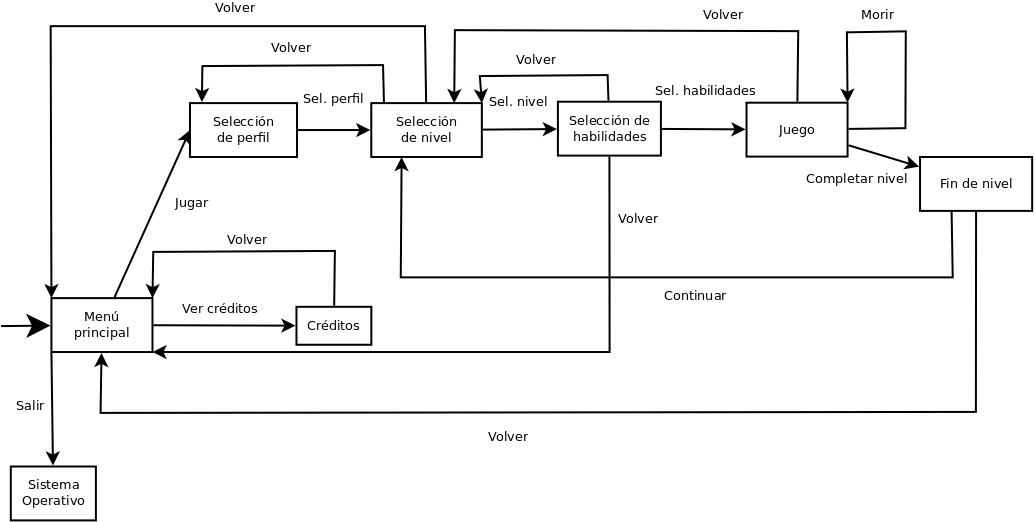
\includegraphics[width=\textwidth]{img/flowchart.png} 
    \caption{Diagrama de flujo de pantallas en el juego}
    \label{img:flowchart}
\end{figure}

\clearpage

\subsection{Menú principal}
\label{sec:ui-menu}

\paragraph{}
A continuación el boceto de la pantalla de \menu:

\begin{figure}[H]
    \centering
        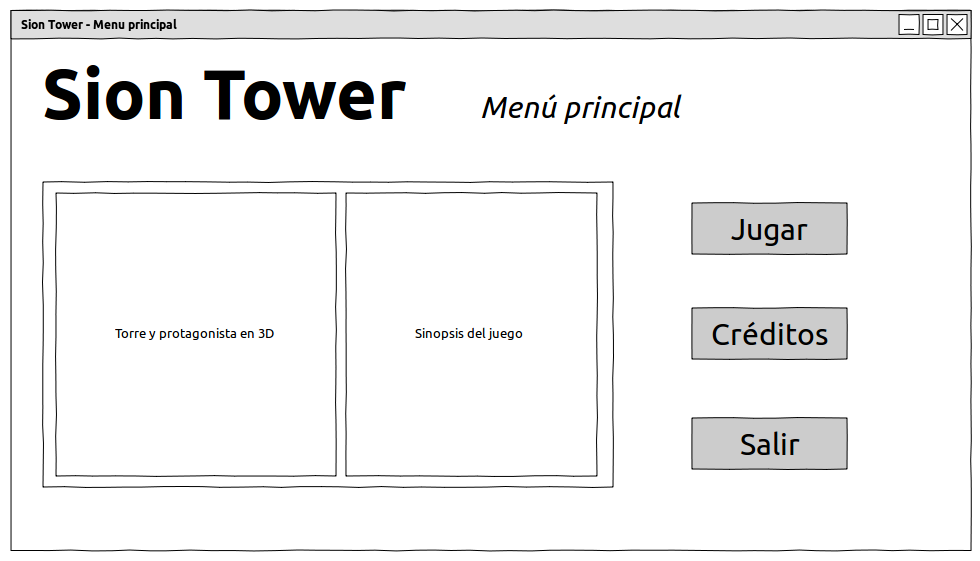
\includegraphics[width=\textwidth]{img/menu-principal.png} 
    \caption{Boceto del menú principal}
    \label{img:menu-principal}
\end{figure}

\paragraph{}
Lista y descripción de todos sus componentes.

\begin{itemize}
    \item \textbf{Botón jugar}: al pulsarlo lleva a la pantalla \selperfil.
    \item \textbf{Botón créditos}: al pulsarlo lleva a la pantalla \creditos.
    \item \textbf{Botón salir}: al pulsarlo nos lleva de vuelta al Sistema Operativo.
    \item \textbf{Torre y protagonista}: vista 3D de la torre (\juego) y del
    protagonista a modo de ambientación.
    \item \textbf{Sinopsis}: texto con una breve introducción a la historia
    del juego.
\end{itemize}

\clearpage

\subsection{Créditos}
\label{sec:ui-creditos}

\paragraph{}
A continuación el boceto de la pantalla de \creditos:

\begin{figure}[H]
    \centering
        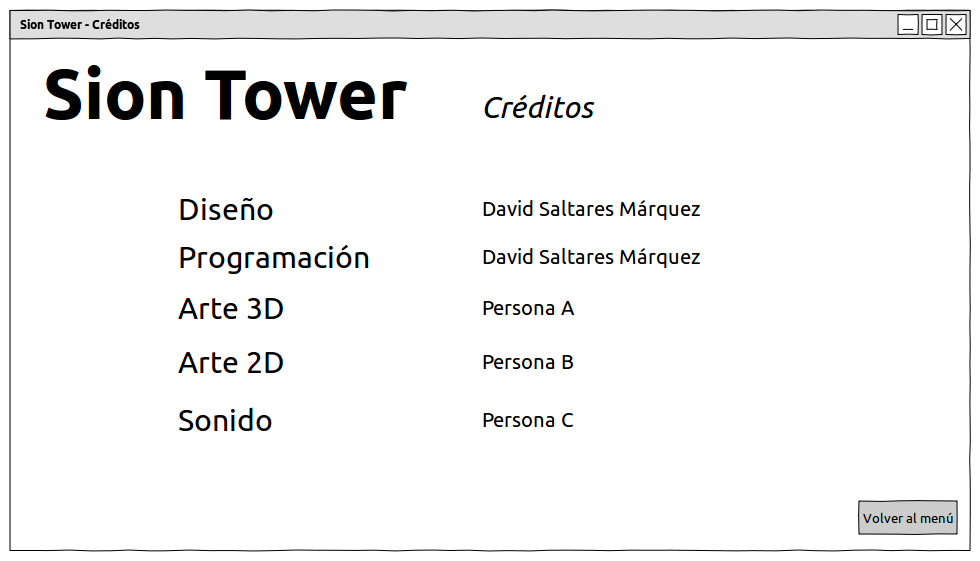
\includegraphics[width=\textwidth]{img/creditos.png} 
    \caption{Boceto de la pantalla de cŕeditos}
    \label{img:creditos}
\end{figure}

\paragraph{}
Lista y descripción de todos sus componentes.

\begin{itemize}
    \item \textbf{Panel}: texto con los componentes del equipo de desarrollo.
    \item \textbf{Botón menú}: al pulsarlo volvemos al \menu.
\end{itemize}

\clearpage

\subsection{Selección de perfil}
\label{sec:ui-perfil}

\paragraph{}
A continuación el boceto de la pantalla de \selperfil:

\begin{figure}[H]
    \centering
        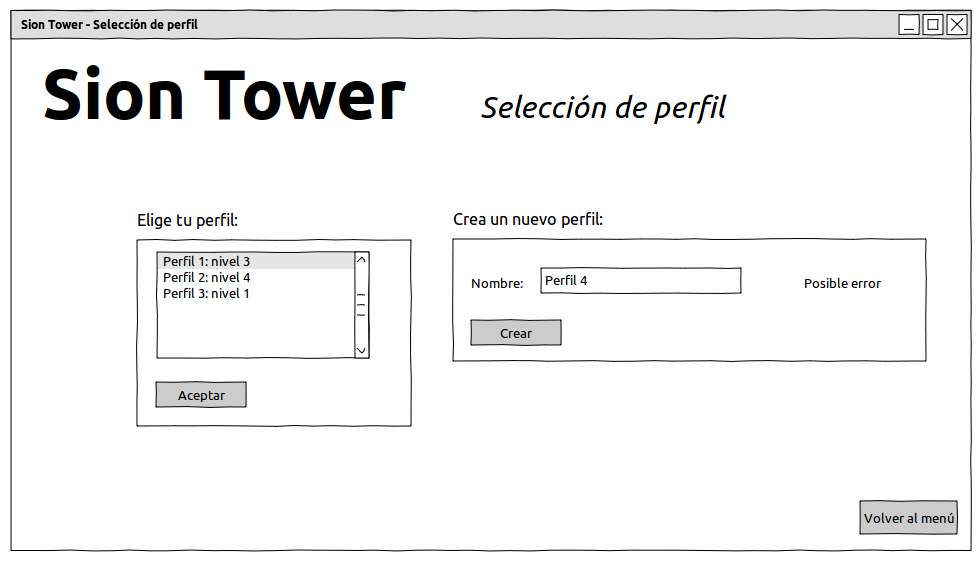
\includegraphics[width=\textwidth]{img/sel-perfil.png} 
    \caption{Boceto de la pantalla de selección de perfil}
    \label{img:sel-perfil}
\end{figure}

\paragraph{}
Lista y descripción de todos sus componentes.

\begin{itemize}
    \item \textbf{Lista de perfiles}: lista con los perfiles guardados
    hasta el momento. Se muestra el nombre del perfil y el nivel alcanzado.
    \item \textbf{Botón aceptar}: al pulsarlo se toma el perfil seleccionado
    y vamos a la pantalla de \selnivel.
    \item \textbf{Crear perfil}: etiqueta y caja de texto para introducir
    el nombre del nuevo perfil.
    \item \textbf{Botón crear}: crea un perfil nuevo con el nombre que contiene
    la caja de texto. Si el perfil existe o no se ha introducido un nombre,
    se muestra un error.
    \item \textbf{Etiqueta error}: muestra el posible mensaje de error
    al tratar de añadir un nuevo perfil.
    \item \textbf{Botón menú}: al pulsarlo volvemos al \menu.
\end{itemize}

\clearpage

\subsection{Selección de nivel}
\label{sec:ui-selnivel}

\paragraph{}
A continuación el boceto de la pantalla de \selnivel:

\begin{figure}[H]
    \centering
        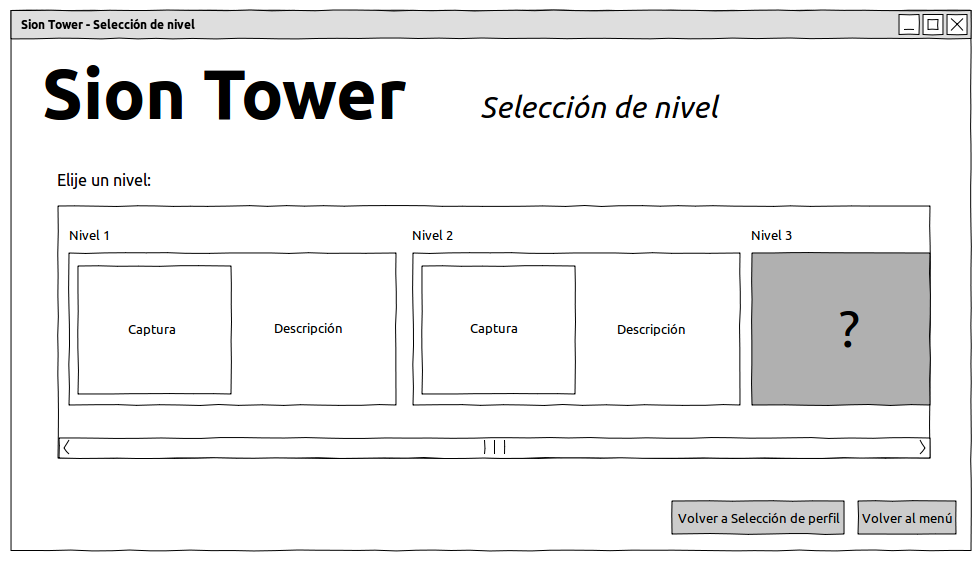
\includegraphics[width=\textwidth]{img/sel-nivel.png} 
    \caption{Boceto de la pantalla de selección de nivel}
    \label{img:sel-nivel}
\end{figure}

\paragraph{}
Lista y descripción de todos sus componentes.

\begin{itemize}
    \item \textbf{Lista de niveles}: bloque con barra de desplazamiento
    horizontal que contiene una caja por cada nivel del juego.
    \item \textbf{Bloque nivel}: cada nivel está representado por un bloque
    que contiene: el nombre del nivel, una pequeña captura y una descripción con
    los avances de la historia. Si el nivel está desbloqueado se mostrará
    con normalidad, si aún no podemos acceder aparecerá un bloque oscuro
    con una interrogación. Para seleccionar un nivel haremos click sobre su
    bloque y pasaremos a la pantalla de \selhabilidad.
    \item \textbf{Botón perfil}: al pulsarlo volvemos a la pantalla \selperfil.
    \item \textbf{Botón menú}: al pulsarlo volvemos al \menu.
\end{itemize}

\clearpage

\subsection{Selección de habilidades}
\label{sec:ui-habilidades}

\paragraph{}
A continuación el boceto de la pantalla de \selhabilidad:

\begin{figure}[H]
    \centering
        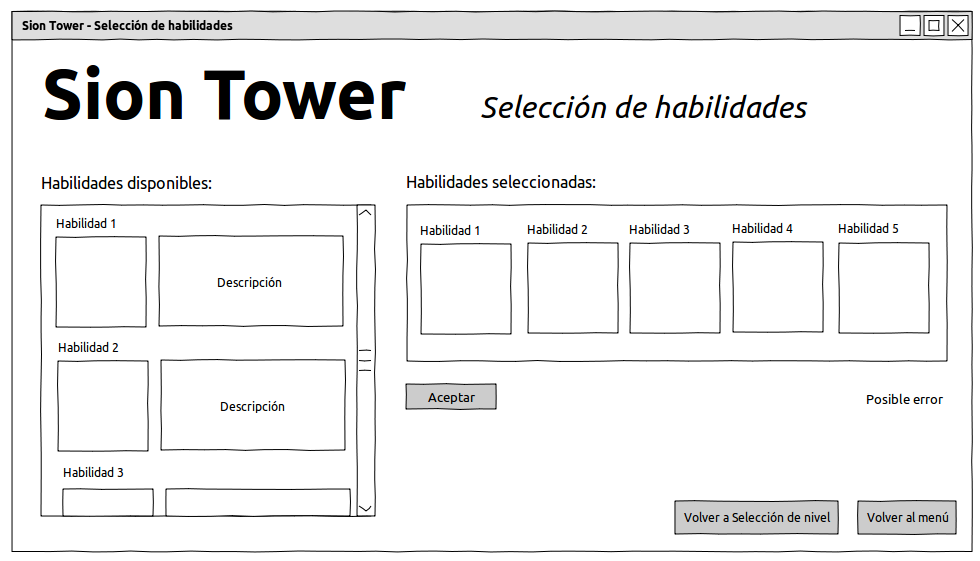
\includegraphics[width=\textwidth]{img/sel-hab.png} 
    \caption{Boceto de la pantalla de selección de habilidades}
    \label{img:sel-hab}
\end{figure}

\paragraph{}
Lista y descripción de todos sus componentes.

\begin{itemize}
    \item \textbf{Habilidades disponibles}: bloque con barra de desplazamiento
    vertical que contiene las habilidades que ha conseguido desbloquear el
    \jugador.
    \item \textbf{Bloque habilidad}: cada habilidad está formada por un bloque
    que contiene su nombre, un icono y una descripción. Al pulsar sobre una habilidad
    se añade automáticamente a la lista de habilidades seleccionadas y queda
    bloqueada en color gris. Si no quedan slots libres, se muestra el error.
    \item \textbf{Bloque seleccionadas}: contiene los slots con las habilidades
    seleccionadas hasta el momento. De cada habilidad sólo se muestra el nombre
    y el icono.
    \item \textbf{Etiqueta error}: se muestra el mensaje de error si no quedan
    slots libres.
    \item \textbf{Botón aceptar}: al pulsarlo avanzamos hacia la pantalla de \nivel.
    \item \textbf{Botón nivel}: al pulsarlo volvemos a la pantalla \selnivel.
    \item \textbf{Botón menú}: al pulsarlo volvemos al \menu.
\end{itemize}

\clearpage

\subsection{Nivel}
\label{sec:ui-nivel}

\paragraph{}
A continuación el boceto de la pantalla de \nivel:

\begin{figure}[H]
    \centering
        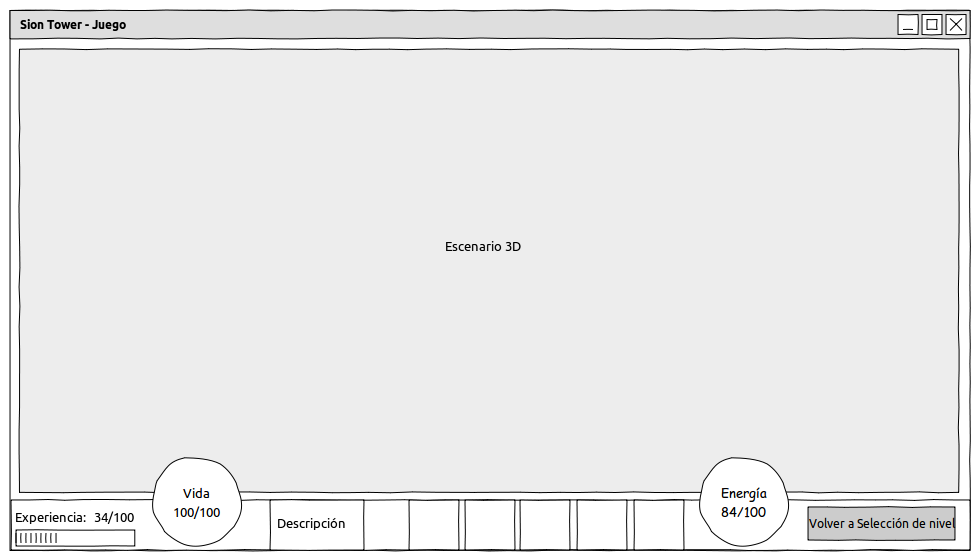
\includegraphics[width=\textwidth]{img/juego.png} 
    \caption{Boceto de la pantalla de juego}
    \label{img:juego}
\end{figure}

\paragraph{}
Lista y descripción de todos sus componentes.

\begin{itemize}
    \item \textbf{Escenario 3D}: panel de juego.
    \item \textbf{Experiencia}: etiquetas con la experiencia actual
    y la necesaria para alcanzar la siguiente habilidad. Incluye
    una barra de progreso.
    \item \textbf{Vida}: bola de contenido verde cuyo nivel varía
    según la cantidad de vida que se posee. Tiene inscrito encima el valor.
    \item \textbf{Energía}: bola de contenido azul cuyo nivel varía
    según la cantidad de energía que se posee. Tiene inscrito encima el valor.
    \item \textbf{Habilidades}: icono de las habilidades disponibles. Si
    no se tiene suficiente energía para utilizar una, ésta aparecerá
    en un tono grisáceo. Al pasar el ratón por encima de algunas, aparece
    su descripción en el recuadro de la izquierda. Para activar la habilidad,
    hacemos click sobre ella.
    \item \textbf{Descripción}: contiene la descripción de la habilidad
    activa.
    \item \textbf{Botón nivel}: al pulsarlo volvemos a la pantalla \selnivel.
\end{itemize}

\clearpage

\subsection{Fin de nivel}
\label{sec:ui-finnivel}

\paragraph{}
A continuación el boceto de la pantalla de \finnivel:

\begin{figure}[H]
    \centering
        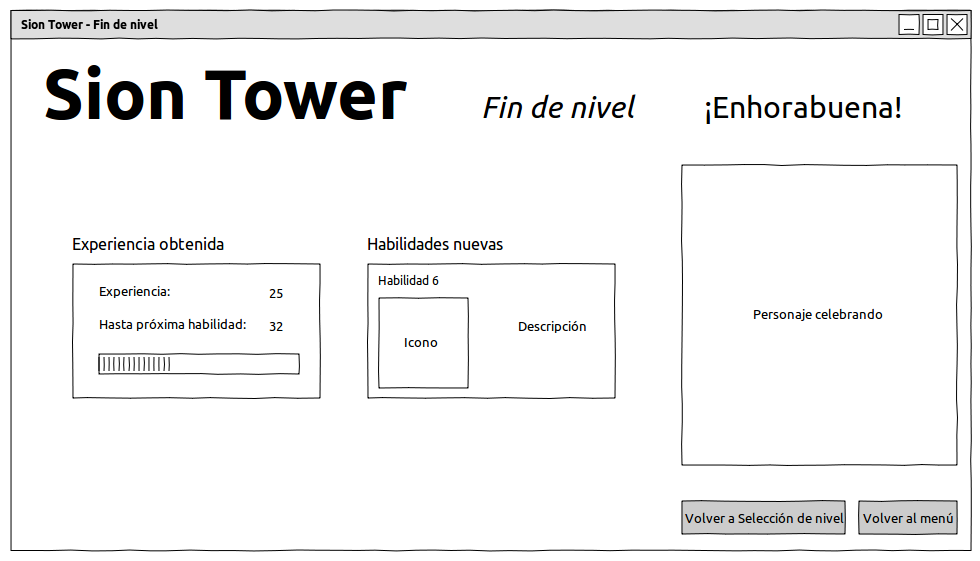
\includegraphics[width=\textwidth]{img/fin-nivel.png} 
    \caption{Boceto de la pantalla de fin de nivel}
    \label{img:fin-nivel}
\end{figure}

\paragraph{}
Lista y descripción de todos sus componentes.

\begin{itemize}
    \item \textbf{Experiencia}: bloque que muestra la experiencia obtenida
    en ese nivel y la experiencia restante para desbloquear la próxima habilidad.
    \item \textbf{Habilidad nueva}: bloque que, en el caso se haber desbloqueado
    una habilidad la mostrará (nombre, icono y descripción). 
    \item \textbf{Personaje}: protagonista en 3D celebrando la victoria.
    \item \textbf{Botón selección de nivel}: al pulsarlo volvemos a la pantalla \selnivel.
    \item \textbf{Botón menú}: al pulsarlo volvemos al \menu.
\end{itemize}

\clearpage

\section{Arte}
\label{sec:arte}
% Objetivo
\paragraph{}
\juego debe tener un carácter alegre a la vez que tenso y épico. Para el
joven protagonista es todo un reto defender la torre sagrada pero aún es inexperto
y no ha perdido su inocencia. Algo similar ocurre en la saga \emph{The Legend
of Zelda}. Los colores deben ser vivos, los modelos muy básicos y la música
acorde con el desenfadado conjunto.

\paragraph{}
A continuación enumeramos los recursos necesarios:

\subsection{Arte 2D}

\paragraph{}
Todas las imágenes deberán estar en formato \emph{.png} además de en el
formato propio del programa con el que se crearon (\emph{.psd} o \emph{.xcf})
para posibles futuras modificaciones. El fichero de trabajo siempre debe
tener una calidad superior a la requerida en el juego.

\paragraph{}
Interfaz

\begin{itemize}
    \item \emph{Logo}: logo con el texto `Sion Tower' siguiendo los requisitos
    anteriormente expuestos. Estilo medieval, mágico y colorido.
    \item \emph{Plantilla para la GUI}: la interfaz de usuario se desarrollará
    bajo CEGUI o similares. Estas bibliotecas trabajan con plantillas,
    es necesario crear una personalizada.
    \item \emph{Puntero}: puntero del ratón, podría ser una mano de mago
    con o sin varita.
    \item \emph{Icono `Bola de fuego'}: imagen cuadrada con una bola de fuego.
    \item \emph{Icono `Furia de Gea'}: imagen cuadrada con un icono de un
    poder relacionado con la naturaleza.
    \item \emph{Icono `Ventisca'}: imagen cuadrada con un hechizo de frío.
    Por ejemplo, lanzando estalactitas.
    \item \emph{Icono `Panel de pinchos'}: imagen cuadrada con una plancha
    de pinchos.
    \item \emph{Icono `Muro mágico'}: imagen cuadrada con un muro semitransparente.
    \item \emph{Icono `Señuelo'}: imagen cuadrada con una especie de reliquia
    dorada (simulando la real).
    \item \emph{Bola de vida}: recipiente esférico que se rellena de color
    rojo indicando el nivel de vida del personaje.
    \item \emph{Bola de energía}: recipiente esférico que se rellena de color
    azul indicando la energía mágica que posee el personaje.
    \item \emph{Cartel de comienzo}: imagen con el texto ¡Ya vienen! que
    se mostrará al comienzo de cada nivel.
    \item \emph{Cartel de victoria}: imagen con el texto ¡Victoria! que
    aparecerá cuando completemos un nivel con éxito.
    \item \emph{Cartel de Game Over}: imagen con el texto Game Over...
    a mostrar cuando el \jugador pierda una partida.
\end{itemize}

\paragraph{}
Texturas

\begin{itemize}
    \item Cada modelo 3D debe tener su textura.
    \item \emph{Cielo estrellado}: fondo que aparecerá en la escena de la torre
    (menú principal).
\end{itemize}

\subsection{Arte 3D}

\paragraph{}
Todos los modelos 3D deben guardarse en el formato \emph{.blend} de Blender
o en el del software correspondiente. Posteriormente se producirá a su conversión
para hacerlos compatibles con el motor.

\paragraph{}
Todos los personajes poseen las animaciones: correr, atacar, recibir daño,
morir y celebrar.

\begin{itemize}
    \item \emph{Personaje}
    \item \emph{Goblin}
    \item \emph{Diablillo}
    \item \emph{Gólem}
    \item \emph{Araña}
    \item \emph{Torre y entorno}: modelo 3D con la torre y un terreno cercano,
    es la escena que se mostrará en el menú principal.
    \item \emph{Reliquia}: reliquia sagrada que hay que proteger en cada nivel.
    Podría ser un objeto en un pedestal.
    \item \emph{Muro invisible} 
    \item \emph{Panel de pinchos}
    \item \emph{Suelo}
    \item \emph{Pared}
    \item \emph{Puerta}
    \item \emph{Mesa}
    \item \emph{Silla}
    \item \emph{Antorcha}
    \item \emph{Columna}
    \item \emph{Armario}
\end{itemize}

\subsection{Audio}

\paragraph{}
De nuevo, siempre es necesario guardar y entregar el proyecto del fichero
de audio en el formato que use el software con el que se produce. La música
se convertirá a \emph{.ogg} mientras que los efectos de sonido estarán
en \emph{.wav}.

\paragraph{}
Música

\begin{itemize}
    \item \emph{Menú principal}: música de aventura y tensión aunque más
    relajada que la correspondiente a los niveles. En el menú aparecerá la torre de noche
    a modo de preámbulo de la invasión por lo que la música debe ser acorde.
    Por supuesto, debe invitar a comenzar una partida.
    \item \emph{Juego}: música animada e intensa que debe provocar en el
    \jugador sensación de tensión.
    \item \emph{Victoria}: música breve que sonará cuando completemos un nivel.
    Debe ser alegre y hacer que el \jugador se sienta recompensado.
    \item \emph{Game Over}: pieza muy breve de derrota con un tinte cómico,
    para restarle gravedad a la partida (que el \jugador piense que haber
    perdido una vez no es tan terrible).
\end{itemize}

\paragraph{}
Efectos

\begin{itemize}
    \item \emph{Navegar por opción}: al pasar el ratón por encima de alguna
    opción.
    \item \emph{Seleccionar opción}: al hacer click con el ratón sobre algún
    elemento.
    \item \emph{Opción no permitida}: pequeña advertencia sonora indicando que
    una acción no puede ser llevada a cabo.
    \item \emph{`Bola de fuego'}: efecto de llamarada
    \item \emph{`Furia de Gea'}: efecto de naturaleza, bosque, rocas...
    \item \emph{`Ventisca'}: viento congelado o cristales cortando el viento.
    \item \emph{Goblin}: risa maliciosa que emitirán los enemigos de tipo.
    \item \emph{Diablillo}: gruñido.
    \item \emph{Gólem}: ruido bruto y pesado.
    \item \emph{Araña}: seseo o ruido propio de un insecto.
    \item \emph{Espadazo}: sonido de una espada cortando el aire.
    \item \emph{Arañazo}: garras del Diablillo.
    \item \emph{Golpe}: golpe producido por el Gólem.
    \item \emph{Ataque araña}: ruido del ataque de la araña.
    \item \emph{Daño Goblin}: sonido al herir al Goblin.
    \item \emph{Daño Diablillo}: sonido al herir al Diablillo.
    \item \emph{Daño Gólem}: sonido al herir al Gólem.
    \item \emph{Daño Araña}: sonido al herir a la araña.
    \item \emph{Daño personaje}: sonido cuando el personaje es dañado.
\end{itemize}


\end{document}
